\documentclass[12pt,a4paper,ngerman]{scrartcl}

%% Laden der benoetigten Pakete:

\usepackage[utf8]{inputenc} %% West- & Mitteleuropa-Kodierung 

\usepackage{babel}% umfangreiches Sprachpaket (Silbentrennung, Gliederungen usw.)

\usepackage{graphicx}% Graphikpaket (fuer PNG,GIF,JPG)

\usepackage[caption=false]{subfig}% Mehrfachabbildungen

\usepackage{float,rotating}%Option [H] fuer fixe Position; Drehung von Abbildungen etc.

\usepackage{array,booktabs}%erweiterte Moeglichkeiten zur Tabellendarstellung

\usepackage{capt-of}

\usepackage{subfig}

\usepackage{wrapfig} %Einbetten von Bildern, Tables etc. in den Text ermöglichen

\usepackage{cite} %Zitieren nach IEEE mit dem Befehl \cite{bla} auf Refrent in thebibliography mit kennung "`bla"'

\usepackage{float} % Bei Gleitobjekten Position mit [H] festsetzen! (Sparsam verwenden!)
%
\usepackage{tikz}%Mindmaps etc.
\usetikzlibrary{mindmap,backgrounds}

% fix citations to be IEEE style
\def\citepunct{], [}
\def\citedash{]--[}

\usepackage{amsmath,amssymb,amsfonts,amsthm}% American Mathematical Society Pakete
\usepackage{textcomp,gensymb}% umfangreiche Pakete fuer Symbole wie:
%% \textmu, \textcelsius, \micro, \ohm, \degree, \celsius
%Kürzen in formeln
\usepackage{cancel}
%Farben ermöglichen
\usepackage{color} 

%\multirow ermöglichen in Tabellen
\usepackage{multirow} 

%Bessere Worttrennung, Kerning ein. 
\usepackage[protrusion=true,expansion=true, kerning]{microtype}

%% Bildunterschriftengestaltung:
\addtokomafont{caption}{\footnotesize}
\addtokomafont{captionlabel}{\bfseries}
\usepackage[pdftex]{hyperref}

\newtheorem{bsp}{Beispiel}[section] %Beispielumgebung, zählschema: Kapittelnummer.Beispielnummer

\setcapwidth[l]{1\linewidth} %Captions unter Tabellen, Bildern etc. Linksbündig und wenn nötig die gersame Seitenbreite

%Einzelzeilen oben und unten unterbinden ("`Hurenkinder"' und "`Schusterjungen"')
\clubpenalty = 10000
\widowpenalty = 10000 
\displaywidowpenalty = 10000

%% Kopf- und Fusszeilengestaltung:
\usepackage{fancyhdr}
\pagestyle{fancy}%Seitenstil mit Kopf- und Fußzeilen
%\lhead{Modul 2} % MODUL O.Ä. HIER EINTRAGEN
%\chead{Gruppe 2}  % GRUPPE, NAME O.Ä. HIER EINTRAGEN
\rhead{Seite \thepage} \lfoot{} \cfoot{} \rfoot{} %Seitenzahlen in Header ausgeben
\renewcommand{\headrulewidth}{0.2pt} %Größe der Kopfzeile

%Dokumentinformationen (Erscheint, wenn man mit der Maus über dem fertigen PDF schwebt. Erst NACH einsetzen der korrekten Daten einkommentieren, falsche Titel etc. sind peinlich.

\author{William Glover}
\title{Systemtheorie und Regelungstechnik} 

%% Layout-Umdefinitionen für die Titelseite (Zum benutzen Kommentierungen mit % vor den Kommandos entfernen) Umdefinition für das restliche Dokument findet an anderer Stelle statt!

% \renewcommand{\baselinestretch}{1.5} %1.5facher Zeilenabstand
% \renewcommand{\labelitemi}{-} %Spiegelstriche statt Bullets

%% Gestaltung der Titelseite:
\renewcommand\maketitle{
    \begin{titlepage}
        \sffamily
        \thispagestyle{empty}
              
\includegraphics[height=2.5cm]{IMTEK_Logo_Farbe}\hfill
\includegraphics[height=3cm]{Uni_Siegel}
        \par
        \vspace{2cm}
        \begin{center}
            \Huge \textbf{Mitschrieb der Vorlesung ``Systemtheorie und Regelungstechnik''}\\
            (SS 2010)\\[6cm]
            \end{center}
            %\includegraphics[height=7cm]{Bla} % BILD AUF DECKBLATT HIER EINBAUEN 
           
% Tabellarische Auflistung der wichtigen Daten des nachfolgenden Werkes. Nach belieben anpassen.

            \begin{tabular}{l}
                \large Dozent: Dr.-Ing. A. Peter\\
         \end{tabular}
         \\
						\begin{tabular}{ll}
                \large Textsatz von William Glover \\
                \large Stand: \today
            \end{tabular}
        
        
%Leere Seite, damit Inhaltsverzeichnis nicht auf der Rückseite des Deckblattes.(Bei Druckversion, bei Emailabgabe auskommentieren!)

 			 \newpage 
       \thispagestyle{empty}~
       \newpage

%Ende leere Zwischenseite   
 
\end{titlepage}
}

%% Liste fuer Silbentrennung bei komplexen Woertern:
\hyphenation{reibungslos schluss-endlich realisiert ter-min-liche}

%% Layout-Umdefinitionen:
\renewcommand{\baselinestretch}{1.5} %1.5facher Zeilenabstand
% \renewcommand{\labelitemi}{-} %Spiegelstriche statt Bullets
\setlength{\parindent}{0pt} % kein Erstzeileneinzug
\begin{document}
\maketitle %Titelseite setzen
\clearpage %danach neue Seite
\renewcommand{\baselinestretch}{1.5} %1.5facher Zeilenabstand
\thispagestyle{empty} %Header auf Titelseite unterdrücken

\tableofcontents %Inhaltsverzeichnis setzen
\newpage 

%Leere Seite, damit Inhalt nicht auf der Rückseite des Inhaltsverzeichnisses beginnt. (Bei Druckversion, bei Emailabgabe auskommentieren!)
        
        \thispagestyle{empty}~
        \newpage
     
%Ende leere Zwischenseite

\setcounter{page}{2} %Seitenzahl auf 2 setzen

% AB HIER BEGINNEN DIE INHALTE!

\addtocounter{section}{-1}%Counter einstellen, sodass Vorwort Kapitel 0 ist.
\section{Vorwort}

\begin{description}
\item[Systemtheorie, Kybernetik:] Allgemeine, formale Wissenschaft von der Struktur, den Relationen und dem Verhalten dynamischer, insbesondere komplexer Systeme, die gewisse allgemeine Eigenschaften realer Systeme aus den verschiedenen Bereichen der Wirklichkeit widerspiegeln. 
\end{description}

\subsection*{Ziele}

\subsubsection*{Beschreibung dynamischer Systeme}
\begin{description}
\item[Methoden:] Modellierung (z.B. als Blockschaltbild, DGL oder Übertragungsfunktion), Simulation (kostengünstig, ungefährlich), ...
\end{description}

\subsubsection*{Analyse dynamischer Systeme}
Fragestellungen wie z.B. ist das System...
\begin{itemize}
\item ...stabil?
\item ...steuerbar?
\item ...schwingungsfähig?
\end{itemize}

\subsubsection*{Beeinflussung dynamischer Systeme}
Ziel der Systemtheorie ist ein \emph{automatisierter, sicherer, optimaler Betrieb von technischen Systemen}. Dies kann auf zwei Arten erreicht werden
\begin{itemize}
\item \textbf{Regelung (kont. Systemzustände):} Ansteuerung des Systems, sodass die Ausgangsgröße den gewünschten Sollverlauf erreicht
\item \textbf{Steuerung (diskrete Systemzustände):} Bei gestörten oder zum Teil unbekannten Systemen fortlaufende Systembeobachtung und Rückführung.
\end{itemize}

\section{Beschreibung dynamischer Systeme durch das Blockschaltbild (BSB)}

\subsection{Beispiele zum Aufstellen eines BSB}
\begin{bsp}[Füllen eines Behälters]
\end{bsp}
\begin{figure}[H]%In Figure einpacken, damit am ENde der Minipageumgebung genug Abstand zum folgenden Text gelassen wird
\begin{minipage}{0.4\linewidth} 
 \begin{figure}[H]
  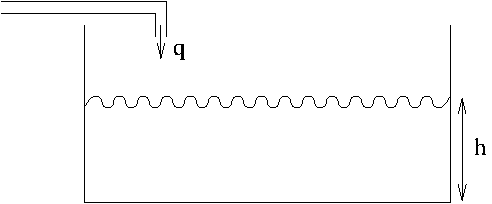
\includegraphics[width=\linewidth]{sysregel_bsp_1} 
  \end{figure}
\end{minipage}
\begin{minipage}{.6\linewidth}
$q(t):\text{Zufluss}$\\
$h(t):\text{Füllstand}$\\
$A:\text{Grundfläche des Behälters}$
\end{minipage}
\end{figure}
Lässt sich hier eine Gesetzmäßigkeit erkennen? Ja! Volumenbilanz:
\begin{equation*}
 v(t)= A \cdot h(t)=\int_0^t{q(\tau)d\tau}(+v_0) 
\end{equation*}
$v_0$: Volumen zum Zeitpunkt $t=0$ \\$\Rightarrow \text{für } v_0 = 0$ gilt:
\begin{equation*}
h(t)=\frac{1}{A}\int_0^t{q(\tau)d\tau}
\end{equation*}
Diese Abhängigkeit lässt sich als ein sogenanntes \emph{Blockschaltbild} wie folgt darstellen:
\begin{figure}[H]
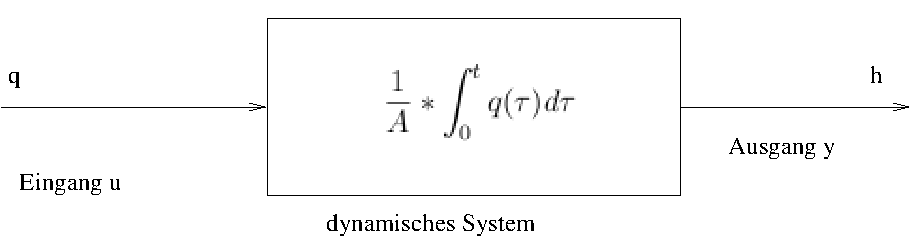
\includegraphics[width=9cm]{sysregel_bsb1}
\end{figure}
Es ist naheliegend, für übliche Operationen eine Bibliothek mit Standard-Blöcken anzulegen, im hier betrachteten Fall z.B. das sogenannte \emph{Integrierglied} (I-Glied).
Die allgemeine Integrationsfunktion
\begin{equation*}
  y(t)=k*\int_0^t{u(\tau)d\tau}
\end{equation*}
wird durch den folgenden Standardblock beschrieben:
\begin{figure}[H]
  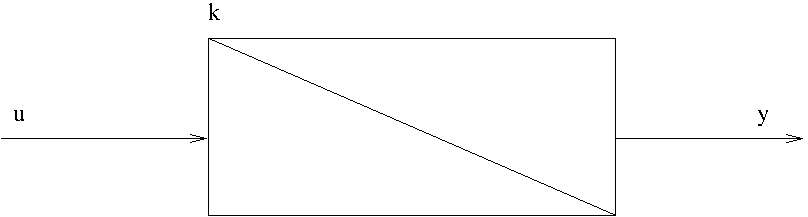
\includegraphics[width=7cm]{sysregel_iglied}
\end{figure}
\begin{bsp}[Erweiterung des Behälters um einen Ablauf]
\end{bsp}
\begin{figure}[H]
\begin{minipage}{0.4\linewidth}
\begin{figure}[H]
  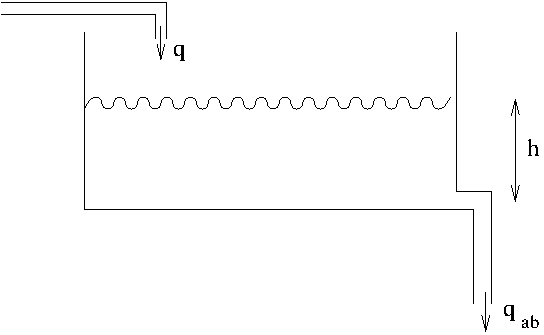
\includegraphics[width=.9\linewidth]{sysregel_bsp_2}  
\end{figure}
\end{minipage}
\begin{minipage}{0.6\linewidth}
$\begin{array}{lll}
q(t)&:&\text{Zufluss}\\
h(t)&:&\text{Füllstand}\\
A&:&\text{Grundfläche des Behälters}\\
q_{ab}(t)&:&\text{Abfluss}
\end{array}$
\end{minipage}
\end{figure}
Für diesen erweiterten Fall wird erneut die Vulumenbilanz aufgestellt:
\begin{equation*}
 v(t)= A \cdot h(t)=\int_0^t{q(\tau)-q_{ab}d\tau}=\int_0^t{u(\tau)d\tau} 
\end{equation*}
Diese lässt sich unter der Annahme, dass $q_{ab}$ von der aktuellen Füllhöhe abhängt, erneut in einem Blockschaltbild folgendermaßen darstellen:
\begin{figure}[H]
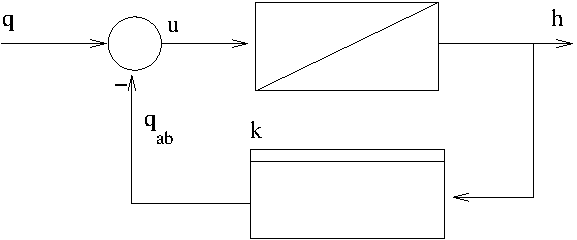
\includegraphics[width=7cm]{sysregel_bsb2}
\end{figure}
Hier wurden bereits zwei weitere, wichtige Standardblöcke eingeführt:
\begin{figure}[H]
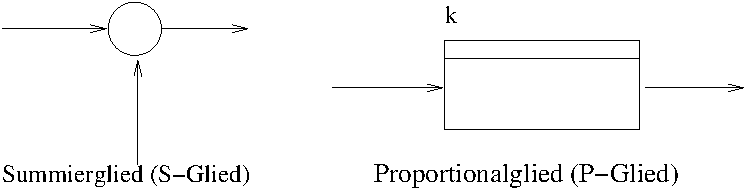
\includegraphics[height=2.5cm]{sysregel_spglied}
\end{figure}
Anhand des Blockschaltbild erkennt man sehr leicht, dass der Füllstand $h(t)$ sich nach einer gewissen Zeit nicht mehr ändert. Der aktuelle Füllstand wird zurückgeführt und vor der Integration von $q(t)$ abgezogen. Sobald gilt $q_{ab}=q$, bleibt $h(t)$ konstant. $u(t)$ wird Null (Stationärer Zustand)!

Da das beschriebene Systemverhalten sehr häufig vorkommt, wird dieses Blockschaltbild zu einem eigenen Standardblock zusammengefasst:
\begin{figure}[H]
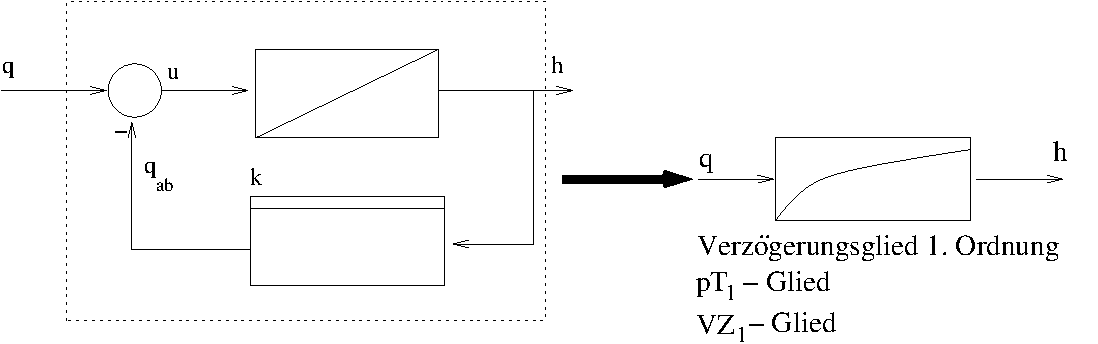
\includegraphics[height=4cm]{sysregel_pt1}
\end{figure}

\begin{bsp}[RC-Glied]
\end{bsp}
\begin{figure}[H]
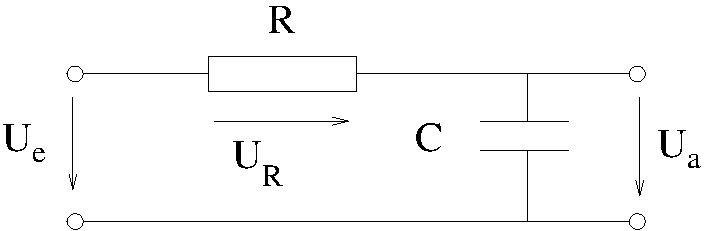
\includegraphics[height=2.5cm]{sysregel_RC}
\end{figure}
Das abgebildete RC Glied wird durch die Gleichungen
\begin{align*}
  \begin{array}{lrlll}
  U_a(t)&=&&\frac{1}{C}*\int_0^t{i(\tau)d\tau}\\
  U_e&=&&U_R+U_a &\Rightarrow U_R=U_e+U_a\\
  \rightarrow i&=&&\frac{U_R}{R}\\
  \Rightarrow i&=&&\frac{1}{R}(U_e-U_a)
 \end{array}
\end{align*}
beschrieben. Für $U_a$ ergibt sich daraus die Gleichung
\begin{equation*}
  U_a(t)=\frac{1}{RC}*\int_0^t{U_e(\tau)-U_a(\tau)d\tau}
\end{equation*}
Auch diese Funktion wird anschließend als Blockschaubild dargestellt:
\begin{figure}[H]
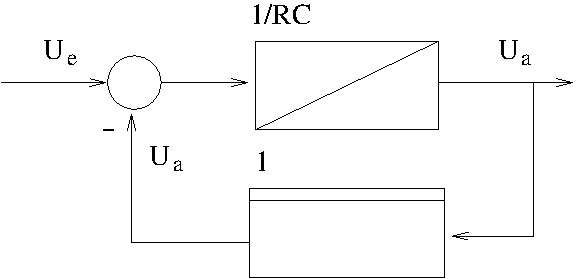
\includegraphics[width=7cm]{sysregel_bsb3}
\end{figure}
\begin{description}
\item[Man erkennt:] Es handelt sich hier ebenfalls um ein Verzögerungsglied 1. Ordnung. Unabhängig von der physikalischen Realisierung haben beide Systeme die gleiche dynamische Struktur!
\end{description}
\begin{bsp}[Erweiterung des Behälters um einen Schwimmer]
\end{bsp}
\begin{minipage}{.4\linewidth}
\begin{figure}[H]
  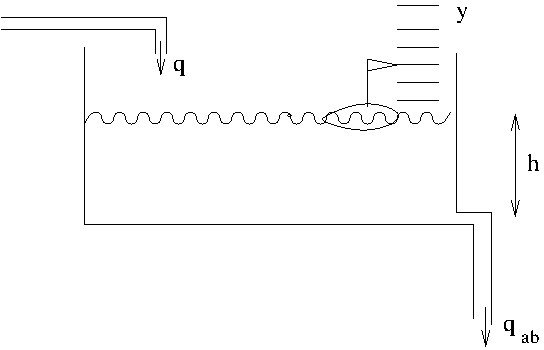
\includegraphics[height=4cm]{sysregel_bsp_4}
\end{figure}
\end{minipage}
\begin{minipage}{.6\linewidth}
\begin{align*}
\begin{array}{lll}
h&:& y $ in Ruhe$\\
m&:& $Masse des Schwimmers$\\
a&:& $Fläche des Schwimmers$\\
\rho&:& $Dichte der Flüssigkeit$\\
\end{array}
\end{align*}
\end{minipage}
Die Auftriebskraft ist gegeben durch $F= (h(t)-y(t))\cdot a \cdot \rho \cdot g$. Durch Umformen lässt sich hieraus die vom Zeiger des Schwimmers angezeigte Skalaposition berechnen:
\begin{equation*}
  F=m \cdot a = m \cdot \ddot{y}=(h(t)-y(t))\cdot a \cdot \rho \cdot g
\end{equation*}
\begin{equation*}
  \Leftrightarrow \ddot{y}= \frac{a \cdot \rho \cdot g}{m}(h(t)-y(t))
\end{equation*}
\begin{equation*}
  \Rightarrow y(t) = \frac{a \cdot \rho \cdot g}{m}\int_0^t{\int_0^\tau{h(T)-y(T)dT}d\tau}
\end{equation*}

\subsubsection*{BSB}

\begin{figure}[H]
  \centering
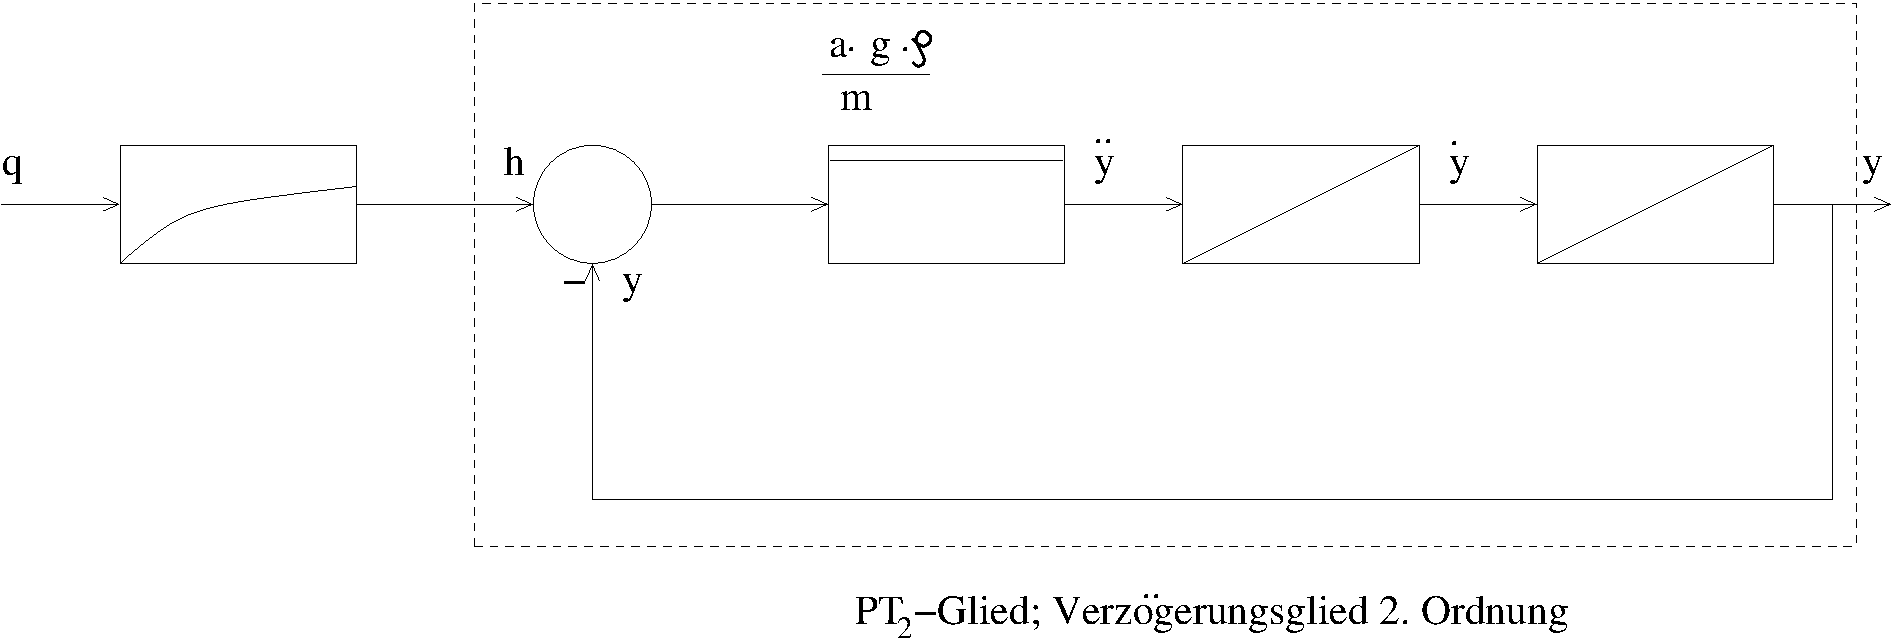
\includegraphics[width=.8\linewidth]{sysregel_bsb5}  
\end{figure}

Auch für das $PT_2$-Glied wird ein eigenes Standardsymbol definiert:
\begin{figure}[H]
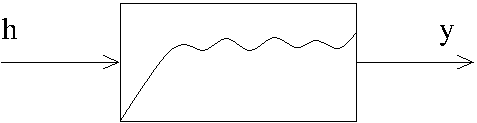
\includegraphics[width=5cm]{sysregel_pt2}
  
\end{figure}


\begin{bsp}[Zuleitung]
\end{bsp}
\begin{figure}[H]
\begin{minipage}{.6\linewidth}
\begin{figure}[H]
 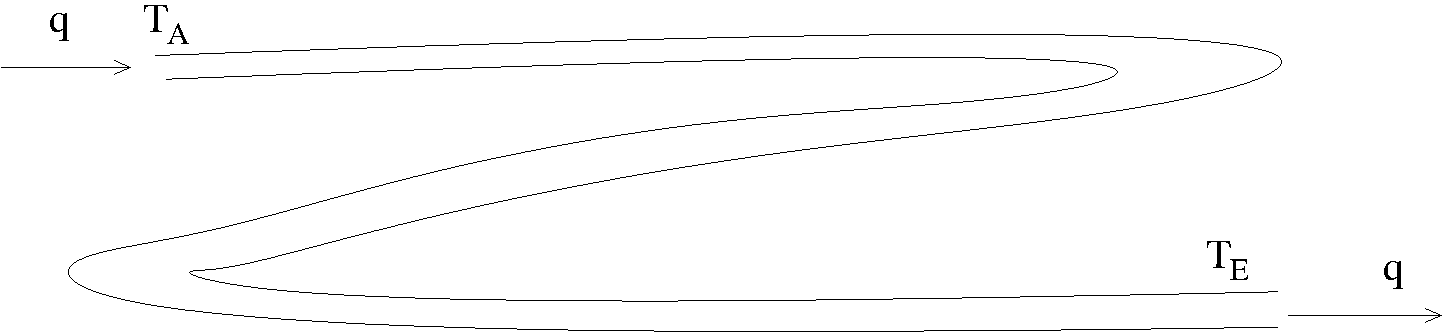
\includegraphics[width=.9\linewidth]{sysregel_bsp_5} 
\end{figure}
\end{minipage}
\begin{minipage}{.4\linewidth}
\begin{tabular}{lll}
$l$&:& Rohrlänge\\
$a$&:&Rohrquerschnitt\\
$v=\frac{q}{a}$&:& Fließgeschwindigkeit
\end{tabular}
\end{minipage}
\end{figure}

Die Zeit, bis eine Probemenge das Rohr durchflossen hat, wird \emph{Totzeit $T_t$} genennt. Sie ist gegeben durch
\begin{equation*}
  T_t=\frac{l}{v}=\frac{l \cdot a}{q}
\end{equation*}
$T_A$ und $T_E$ sind die Temperaturen am Rohranfang bzw. Rohrende. Unter der Annahme, dass das Rohr perfekt isoliert ist, beim Transport also keine Wärme verloren geht, hängen diese beiden Größen über die Sprungfunktion
\begin{equation*}
  T_E(t)=T_A(t-T_t)
\end{equation*}
zusammen. Dieser Zusammenhang wird im Blockschaubild durch das sogenannte \emph{Totzeitglied} dargestellt:
\begin{figure}[H]
  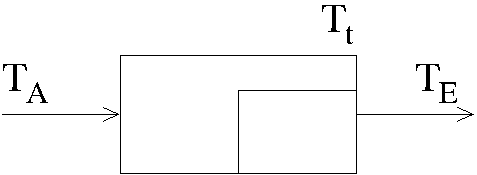
\includegraphics[width=4cm]{sysregel_tglied}
\end{figure}

\subsubsection*{Blockschaltbilder}
\begin{itemize}
\item beschreiben Ursache-Wirkungszusammenhänge in einer allgemeinen Form
\item sind insbesondere bei komplexen Systemen oft übersichtlicher als Darstellungen in Gleichungen
\item lassen sich schrittweise aufbauen und verifizieren
\item sind Basis für numerische Simulationen($\rightarrow$ Simulink)
\end{itemize}

\subsection{Häufig verwendete Übertragungsglieder}

\begin{itemize}
\item \textbf{elementare: }P,I,D,S,$T_t$
\item \textbf{zusammengesetzte: } $PT_1, PT_2$
\item \textbf{nichtlineare: } KL, M
\end{itemize}
In der Vorlesung werden hauptsächlich elementare und zusammengesetzte Übertragungsglieder verwendet!

\subsection{Nichtlineare Glieder und Linearisierung}

\begin{figure}[H]
  \begin{minipage}{.4\linewidth} %Anfang Bildbereich, 0,45 % der Seitenbreite
\begin{figure}[H]
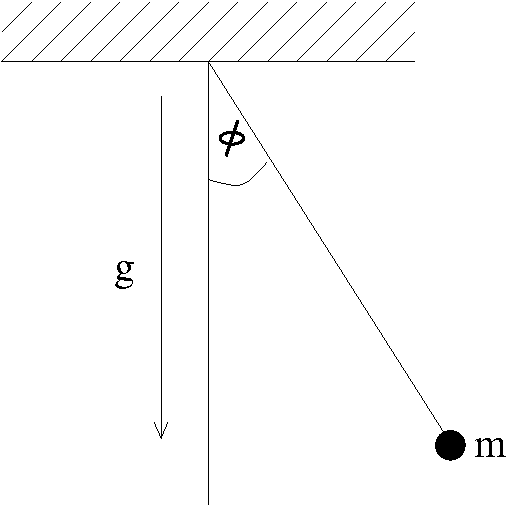
\includegraphics[height=5.5cm]{sysregel_bsp_6} % Hier Bild einfügen
\end{figure}
 \end{minipage}% Ende des Bildbereiches
  \begin{minipage}{.6\linewidth} %Anfang Formelbereich, 0,55 % der Seitenbreite
   \begin{align*}
    &&J*\ddot{\phi}&&=&&&M\\
\rightarrow&& m\cdot l^2 \cdot \ddot{\phi} &&=&&& -m\cdot g \cdot l \cdot sin(\phi)\\
\rightarrow&& l \cdot \ddot{\phi}&&=&&&-g*sin(\phi)\\
\rightarrow&& \ddot{\phi}&&=&&& -\frac{g}{l}sin(\phi)
   \end{align*}
   \begin{tabular}{lll}
$J$&:& Trägheitsmoment\\
$M$&:& Drehmoment
  
   \end{tabular}

\end{minipage}% Ende des Tabellenbereiches
\end{figure}

Erneut wird das Blockschaltbild aufgestellt, unter Verwendung des sog. \emph{Kennliniengliedes} (KL-Glied):

\begin{figure}[H]
  \centering
  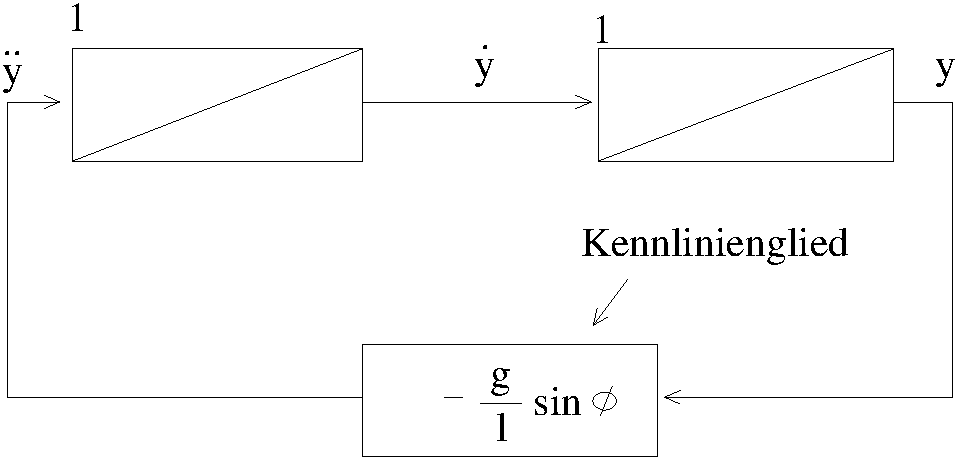
\includegraphics[width=.5\linewidth]{sysregel_bsb4}
\end{figure}

Ein nichtlineares System lässt sich zwar numerisch simulieren, stellt aber ein Problem bei der Analyse oder beim Regelentwurf dar. Als Hilfsmittel wird daher eine Linearisierung im Arbeitspunkt verwendet.
\begin{description}
\item[Arbeitspunkt: ]Betriebszustand eines Systems, in dem die zeitveränderlichen Größen fest sind (stationärer Zustand) und sich das System in einem gewünschten Sollzustand befindet. 
\end{description}
Wird das System nun um den Arbeitspunkt linearisiert, sind die Abweichungen zwischen nichtlinearem und linearem Modell \emph{in der Umgebung um diesen Arbeitspunkt herum }nur klein. Bei zu großer Abweichung vom Arbeitspunkt bildet das lineare Modell das nichtlineare nur unzureichend ab. Der Arbeitspunkt muss dann verändert/neu bestimmt werden. 

\subsubsection*{Linearisierung eines KL-Gliedes}
\begin{figure}[H]
\center
  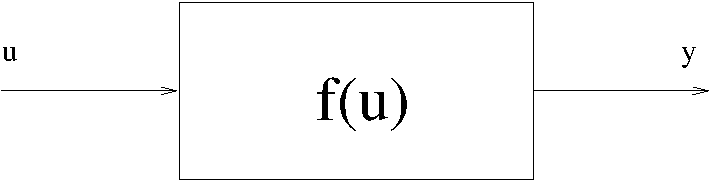
\includegraphics[width=6cm]{sysregel_klglied}
\end{figure}

\begin{eqnarray*}
  y&=&f(u) \\
y_0+ \Delta y &=& f(u_0+ \Delta u)
\end{eqnarray*}
Es wird nun die Taylorreihen-Entwicklung für diese Funktion durchgeführt:
\begin{eqnarray*}
  y_0+\Delta y &=& f(u_0) + [\frac{df(u)}{du}]_{u_0} \cdot \Delta u + \dots\\
  \Rightarrow y_0& =& f(u_0)\\ \Delta y &=&[\frac{df(u)}{du}]_{u_0} \cdot \Delta u + \dots \text{ (Nichtlineare Terme werden Vernachlässigt!)}
\end{eqnarray*}
z.B. $y=sin(\phi)$: Linearisierung um den Arbeitspunkt $\phi_0 =0$
\begin{eqnarray*}
y_0 &=& 0\\
\Delta y&=& [cos(\phi)]_{\phi_0 =0} \cdot \Delta \phi\\
\Rightarrow T_y &=& 1 \cdot \Delta \phi 
\end{eqnarray*}

\begin{figure}[H]
\center
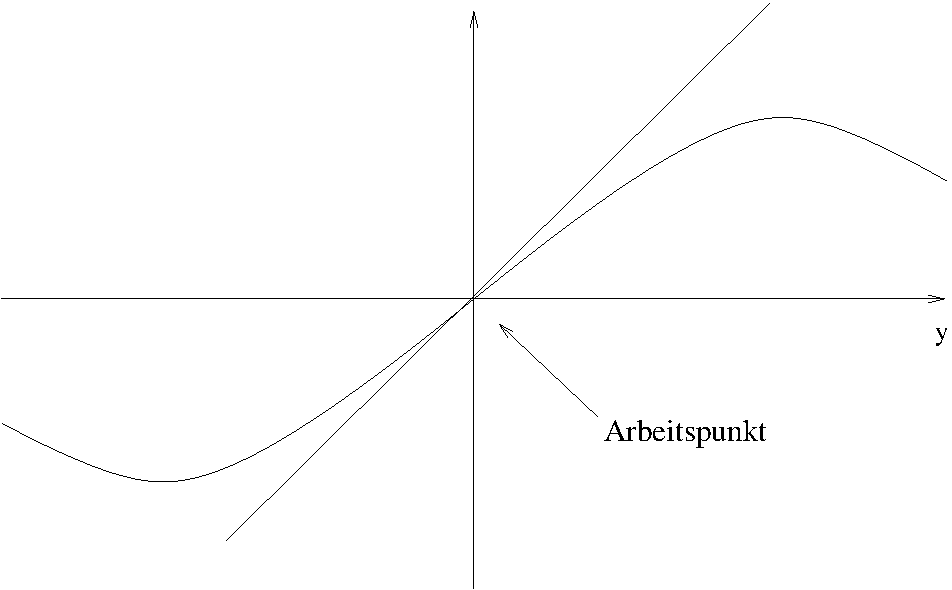
\includegraphics[width=8cm]{sysregel_linear}
\end{figure}

\section{Systembeschreibung im Zeitbereich}

\subsection{Differentialgleichungen}

\subsubsection{Aufstellen der DGL}

Die Differentialgleichung eines Systems kann auf 2 Arten bestimmt werden:
\begin{itemize}
\item aus den physikalischen Gleichungen, z.B.:
  \begin{itemize}
  \item Bewegungsgleichungen: $F(t)=m \cdot \ddot{x}(t)$ ; $M(t)=J \cdot \ddot{\phi}$
  \item Bilanzierung von Volumen: $q_{zu}(t)-q_{ab}(t)=\dot{v}(t)$ 
  \end{itemize}
\item aus dem Blockschaubild:
  \begin{itemize}
  \item eventuell Hilfsgrößen einführen (z.B. Ausgang von S-Gliedern,\dots
  \item Entgegen der Signalflussrichtung durch das BSB gehen und Funktionsbeziehungen der Blöcke auswerten
   \end{itemize}
\end{itemize}
\textbf{Bsp.:} $PT_1$-Glied

   \begin{figure}[H]
     \centering
     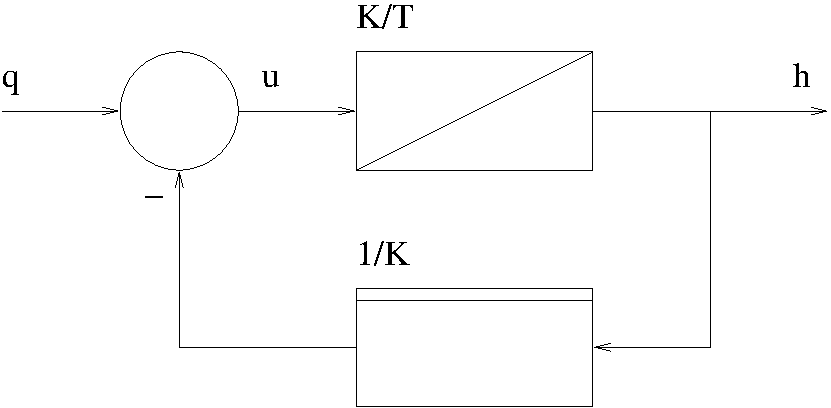
\includegraphics[width=.5\linewidth]{sysregel_bsb6}
   \end{figure}
   \begin{math}
     \begin{array}{llll}
       &h(t)&=&\frac{K}{T}\int_0^t{u(\tau)d\tau}\\
     \rightarrow&\dot{h}(t)&=&\frac{K}{T}\cdot u(t)\\
     &u(t)&=&q-\frac{1}{K}\cdot h(t)\\
     \Rightarrow&\dot{h}(t)&=&\frac{K}{T}\cdot (q(t)-\frac{1}{K} \cdot{h}(t))\\
     \Rightarrow&\frac{1}{T}\cdot h(t)+\dot{h}(t)&=&\frac{K}{T}\cdot q(t)\\
     \Rightarrow&\underbrace{h(t)+T\cdot \dot{h}(t)}_{\text{DGL in }h(t)}&=&\underbrace{k\cdot q(t)}_{\text{Anregung}}\\

     \rightarrow& \multicolumn{3}{l}{\text{homogene DGL, falls }q(t)=0 \text{ (Anregung}=0)}
   \end{array}
  \end{math}

  \subsubsection{Lösung von Differentialgleichungen mit konstanten Koeffizienten}

  \begin{bsp}[Lösung der DGL des $PT_1$-Gliedes]
\end{bsp}
Gegeben ist die Gleichung
\begin{equation*}
  T\cdot \dot{y}(t)+y(t)=k\cdot u(t)
\end{equation*}
mit $y(0)=y_0$ und beliebigem $u(t)$ für $t>0$.
\begin{itemize}
\item \textbf{1. Schritt:} characteristische Gleichung:\\
  \begin{math}
    \begin{array}{llllllll}
      &T\cdot s +1&=&0\\
      \rightarrow&s_1&=&-\frac{1}{T}\\
      \Rightarrow&y_h(t)&=&C_1\cdot y_1(t)&=&c_1*e^{-\frac{t}{T}}&\text{(Formelsammlung)}
    \end{array}
  \end{math}
\item \textbf{2. Schritt:} Variation der Konstanten\\
  \begin{math}
    \begin{array}{lllllllll}
                       &y_p(t)&=&C_1(t)e^{-\frac{t}{T}}\\
      \text{ableiten: }&\dot{y_p}(t)&=&\frac{-C_1(t)}{T}e^{-\frac{t}{T}}+\dot{C_1}(t)e^{-\frac{t}{T}}\\
\multicolumn{4}{l}{\text{In die inhomogene DGL einsetzen:}}\\
&K\cdot u(t)&=&T\cdot (-\frac{\cancel{c_1(t)}}{T}\cdot \cancel{e^{-\frac{t}{T}}}+\dot{C_1}(t)\cdot e^{-\frac{t}{T}})+\cancel{C_1(t)\cdot e^{-\frac{t}{T}}}\\
&\dot{C_1}(t)&=&\frac{K}{T}\cdot e^{\frac{t}{T}}\cdot u(t)\\
\text{Integrieren:}&C_1(t)&=&\int_0^t{\frac{K}{T}\cdot e^{\frac{\tau}{T}}\cdot u(\tau)d\tau}\\
\Rightarrow&y_p(t)&=&[\int_0^t{\frac{K}{T}\cdot e^{\frac{\tau}{T}}\cdot u(\tau)d\tau}]\cdot e^{-\frac{t}{T}}\\
&&=&\int_0^t{\frac{K}{T}\cdot e^{-\frac{t-\tau}{T}}\cdot u(\tau)d\tau}

    \end{array}
  \end{math}
\item \textbf{3. Schritt:} Zusammenfassen zur Gesamtlösung\\
  \begin{math}
    \begin{array}{lll}
      y(t)&=&y_n(t)+y_p(t)\\
          &=&c_1\cdot e^{-\frac{t}{T}}+\int_0^t{\frac{K}{T}\cdot e^{-\frac{t-\tau}{T}}\cdot u(\tau)d\tau}
    \end{array}
  \end{math}
\item \textbf{4. Schritt:} $C_1$ bestimmen\\
  \begin{math}
    \begin{array}{llll}
     &y(0)&=&C_1=y_0\\
     \Rightarrow \text{Lösung:}&y(t)&=&\underbrace{y_0\cdot e^{-\frac{t}{T}}}_{1}+\underbrace{\int_0^t{\frac{K}{T}\cdot e^{-\frac{t-\tau}{T}}\cdot u(\tau)d\tau}}_{2}
    \end{array}
  \end{math}
  \begin{itemize}
  \item \textbf{Formelteil 1} ist die homogene Lösung. Sie ist nur vom Anfangswert $y_0$ abhängig. Man sagt: Sie beschreibt die \emph{freie Bewegung}
  \item \textbf{Formelteil 2} ist die Partikulärlösung. Sie ist nur von der Eingangsfunktion $u(t)$ abhängig. Man sagt: Sie beschreibt die \emph{erzwungene Bewegung}
  \end{itemize}
\end{itemize}

\subsection{Übertragungsverhalten}

\subsubsection{Gewichtsfunktion und Faltung}

Das Übertragungsverhalten von $u(t)$ zu $y(t)$ wird durch den Term
\begin{equation*}
  y(t)=\int\limits_0^t{\frac{K}{T}\cdot e^{\frac{-t-\tau}{T}}\cdot u(\tau)d\tau}
\end{equation*}
definiert. Er beschreibt das Übertragungsverhalten bei verschwindenden Anfangsbedingungen ($y_0=0$). Mit der Funktion
\begin{equation*}
  g(t)=\frac{K}{T}\cdot e^{-\frac{t}{T}}
\end{equation*}
lässt sich das Integral zu
\begin{equation*}
  y(t)=\underbrace{\int\limits_0^t{g(t-\tau)\cdot u(\tau)d\tau}}_{Faltungsintegral}=g(t)*u(t)
\end{equation*}
vereinfachen. Das Zeichen $*$ wird als ``gefaltet mit'' ($g(t)$ gefaltet mit $u(t)$) gelesen. \\
$g(t)$ nennt man \emph{Gewichtsfunktion}. Sie beschreibt das Übertragungsverhalten des Systems vollständig!

\begin{description}
\item[Es gilt:] $g(t)*u(t)=u(t)*g(t)$
\end{description}
Die Gewichtsfunktion $g(t)$ gibt an, mit welchem Gewicht der Wert der Eingangsfunktion $u(t)$ von \emph{zurückliegenden} Zeitpunkten $(t-\tau)$ in den Wert der Ausgangsfunktion $y(t)$ zum \emph{aktuellen} Zeitpunkt $t$ eingeht.\\
\textbf{BILDER FEHLEN!!!}

\subsubsection{Eigenschaften}
\textbf{Lineare} und \textbf{zeitinvariante} Systeme lassen sich durch die Gewichtsfunktion vollständig beschreiben. (Entspricht der linearen DGL mit konstanten Koeffizienten)
\begin{description}
\item[Linearität:] Ein System ist linear, wenn...
  \begin{itemize}
  \item ...das Superpositionsprinzip: $y(t)=g(t)*[u_1(t)+u_2(t)]=g(t)*u_1(t)+ g(t)*u_2(t)$
  \item ...das Verstärkungsprinzip: $y(t)=g(t)*[\alpha \cdot u(t)]= \alpha \cdot[g(t)*u(t)]$
  \end{itemize}
gelten.
\item[Zeitinvarianz:] Das System ist invariant gegenüber Zeitverschiebungen: \\
Aus $y(t)=g(t)*u(t)$ muss für eine beliebige Zeitverschiebung $T$ folgen, dass $y(t-T)=g(t)*u(t-T)$
\item[Kausalität:] Das Ausgang $y(t)$ eines kausalen Systems hängt \emph{nur} vom Verlauf des Eingangs $u(t)$ für Zeiten $t\le t_0$ ab. Das System hängt also nur von vergangenen Eingangswerten ab. Für $g(t)$ kausaler Systeme gilt also:
  \begin{equation*}
    g(t)=0 \text{ für } t<0
  \end{equation*}
\end{description}

\subsubsection{Sprungsantwort und Impulsantwort}

\begin{description}
\item[Sprungantwort:] Auf den Systemeingang wird ein \emph{Einheitssprung} gegeben \textbf{evtl. Bild einfügen!}:
  \begin{equation*}
    u(t)=\sigma (t) =\begin{cases} 0 $ für $t<0\\1 $ für $ t \geq 0\end{cases}
  \end{equation*}
Die Antwort des Systems heißt \emph{Sprungantwort} und wird beschrieben durch
\begin{equation*}
  h(t):=y(t)
\end{equation*}
Mit dem Flächenintegral $y(t)=\int\limits_0^t{g(\tau)\cdot u(t-\tau)d\tau}$ vereinfacht sich das zu
\begin{align*}
  \begin{array}{lll}
    h(t)&=&\int\limits_0^t{g(\tau)\cdot \underbrace{\sigma (t-\tau)}_{=1}d\tau}\\
    h(t)&=&\int\limits_0^t{g(\tau)d\tau}  
  \end{array}
\end{align*}
Die Sprungantwort, genau wie die Gewichtsfunktion, characterisiert das dynamische System vollständig!
\item[Impulsantwort: ] Die Impulsfunktion $\delta (t)$ ist die formale Ableitung des Einheitssprungs.
  \begin{equation*}
    \delta (t)=\frac{d}{dt}\sigma (t) \Leftrightarrow \int\limits_0^t{\delta(\tau)d\tau =\sigma(t)}
  \end{equation*}
Für die Impulsantwort gilt damit:
\begin{equation*}
  \int\limits_0^t{g(\tau)\cdot u(t-\tau)d\tau} =\int\limits_0^t{g(\tau)\cdot \delta(t-\tau)d\tau }=g(t)
\end{equation*}
$\Rightarrow$ Die Gewichtsfunktion $g(t)$ kann auch als Impulsantwort interpretiert werden.

\end{description}

\subsection{Darstellung im Zustandsraum}

\begin{bsp}[System aus 3 verbundenen Wassertanks]
\end{bsp}
\begin{figure}[H]
  \centering
  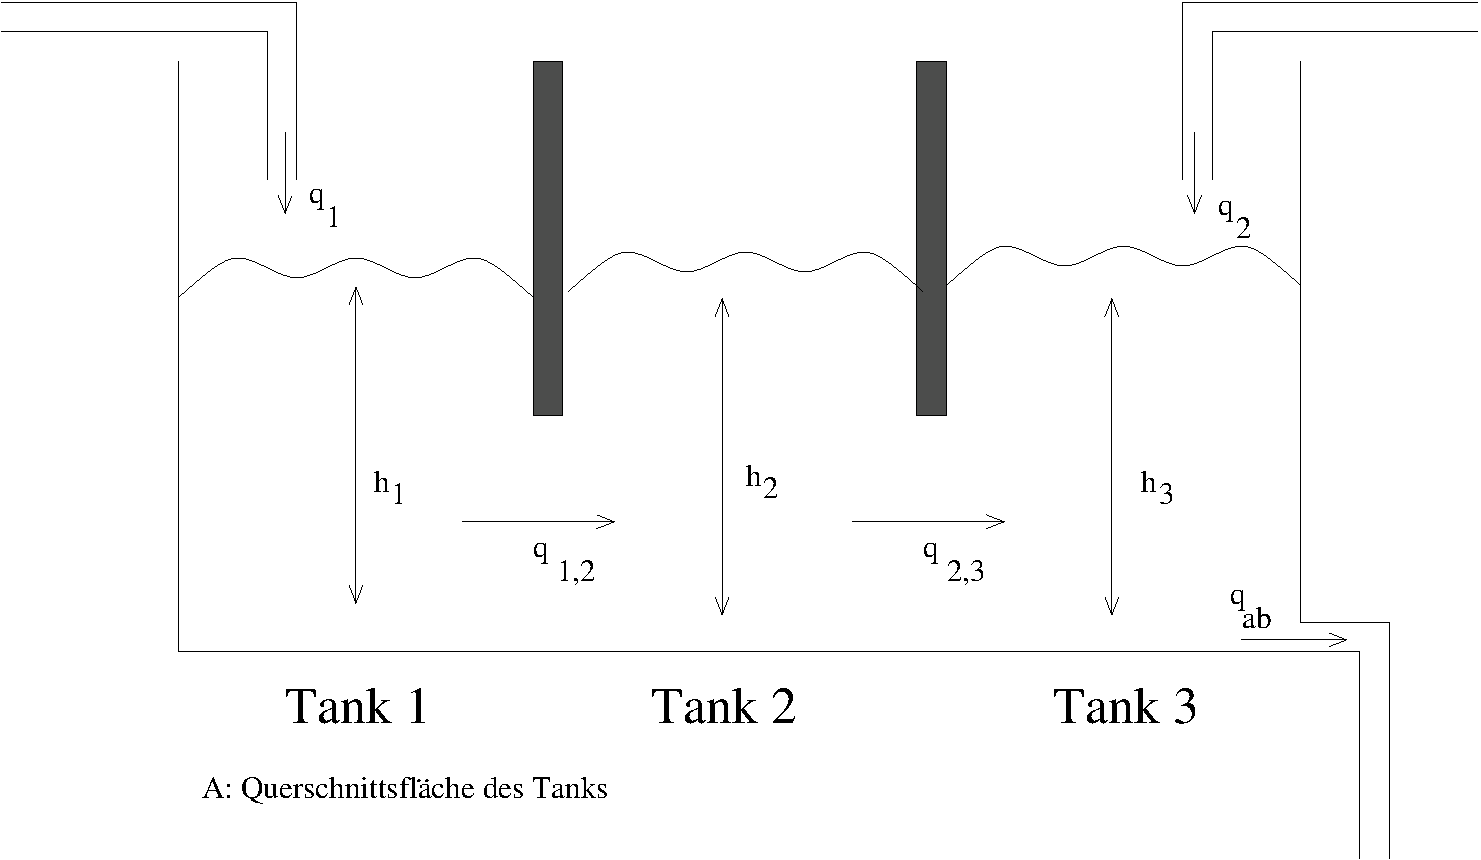
\includegraphics[width=.9\linewidth]{sysregel_bsp_2,2}
\end{figure}
Volumenbilanz:
\begin{align*}
  \begin{array}{llll}
    \text{Tank 1:}&\dot{h_1}&=&\frac{1}{A}(q_1-q_{1,2})\\
    \text{Tank 2:}&\dot{h_2}&=&\frac{1}{A}(q_{1,2}-q_{2,3})\\
    \text{Tank 3:}&\dot{h_3}&=&\frac{1}{A}(q_{2}+q_{2,3}-q_{ab})
  \end{array}
\end{align*}
\begin{description}
\item[Annahme:]Der Ausgleichsfluss zwischen den Tanks ist proportional zur Füllstandsdifferenz: \begin{center}  $q_{1,2}=c\cdot (h_1-h_2);q_{2,3}=c\cdot (h_2-h_3);q_{ab}=ch_3$ \end{center}
\end{description}
\begin{align*}
  \begin{array}{llll}
    \text{damit:}&\dot{h_1}&=&\frac{1}{A}(q_1-ch_1+ch_3)\\
                 &\dot{h_2}&=&\frac{1}{A}(ch_1-2ch_2+ch_3)\\
                 &\dot{h_3}&=&\frac{1}{A}(q_2+ch_2-2ch_3)
  \end{array}
\end{align*}
Kennt man $h_1,h_2,h_3$, so ist der Zustand des Systems zum Zeitpunkt t vollständig bestimmt. $\Rightarrow h_1,h_2,h_3$ sind die Zustandsgrößen des Systems.\\
\textbf{Geometrische Deutung:} $h_1,h_2,h_3$ spannen einen dreidimensionalen Vektorraum auf, den sogenannten \emph{Zustandsraum}.\\
\begin{figure}[H]
  \begin{minipage}{0.5\linewidth}
    \begin{figure}[H]
      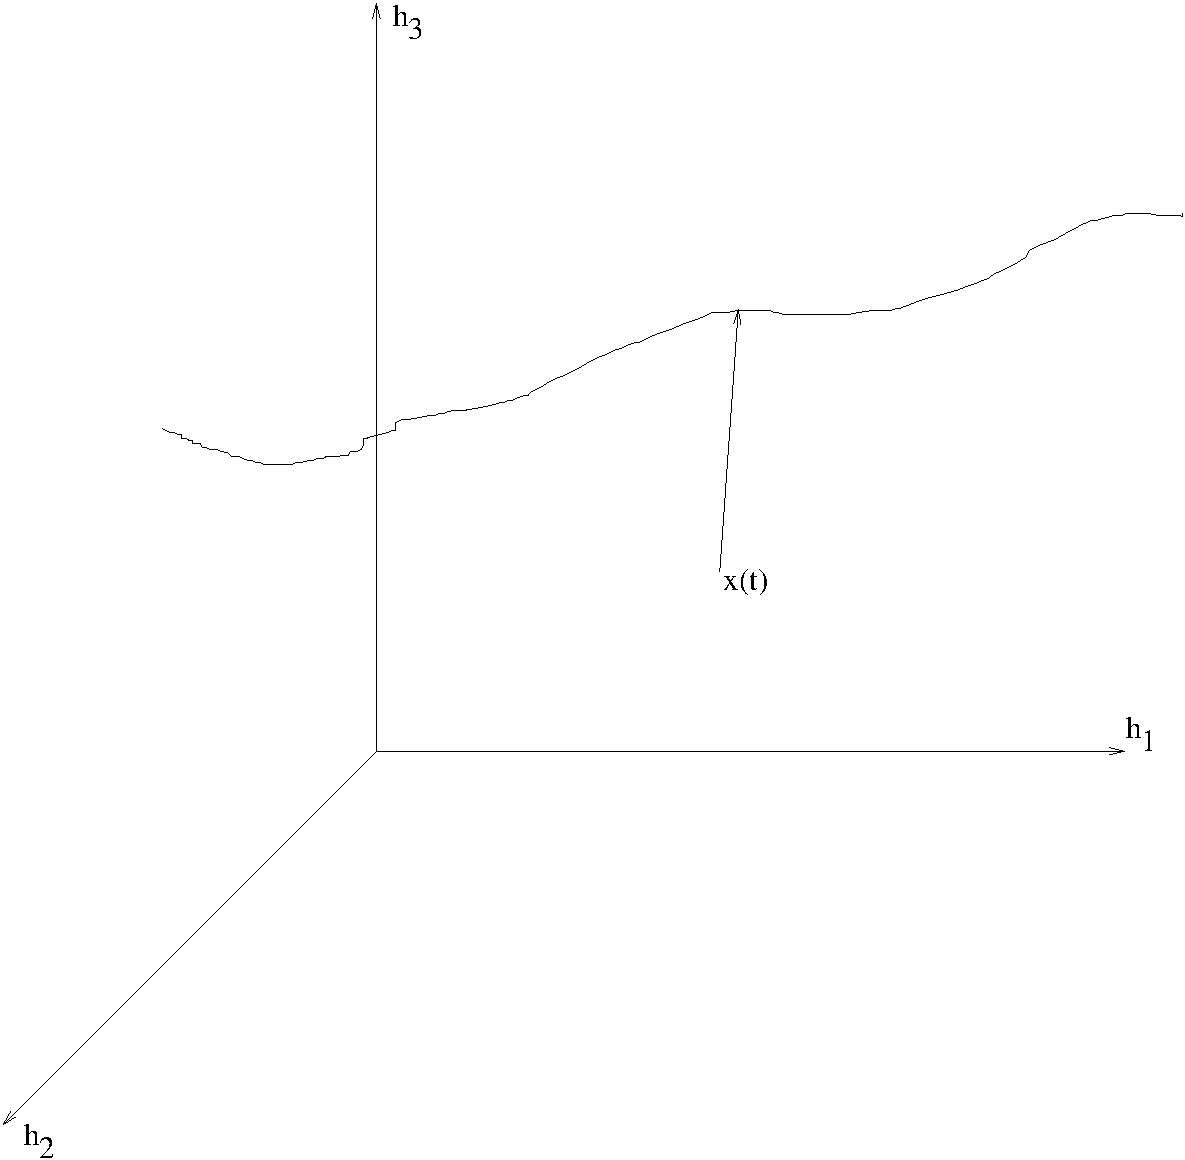
\includegraphics[width=0.9\linewidth]{sysregel_zustandsraum}
    \end{figure}
  \end{minipage}
  \begin{minipage}{0.5\linewidth}
    \[\vec{x}(t): \text{Zustandsvektor}\\\]
    \[\vec{x}(t)=  \begin{pmatrix}
            h_1(t) \\
            h_2(t) \\
            h_3(t) \end{pmatrix} \] 
  \end{minipage}
\end{figure}
Das System wird durch $q_1(t)$ und $q_2(t)$ angeregt, diese sind die \emph{Eingangsgrößen}. Aus ihnen lässt sich der sogenannte \emph{Eingangsvektor} bestimmen:
\begin{equation*}
  \vec{u}(t)=\begin{pmatrix}
                            q_1(t)\\
                            q_2(t)
             \end{pmatrix}
\end{equation*}

\subsubsection*{Verallgemeinerung}

Das Systrem lässt sich durch $n$ Zustände beschreiben:
\[
\vec{x}=
\begin{pmatrix}
x_1\\
x_2\\
\vdots\\
x_n
\end{pmatrix}
\]
Das Systrem besitzt $m$ Eingänge:
\[
\vec{u}=
\begin{pmatrix}
u_1\\
u_2\\
\vdots\\
u_m
\end{pmatrix}
\]
Dieses System lässt sich durch $n$ DGL 1 Ordnung beschreiben:
\[
\left.
\begin{array}{cc}
x_1=f_1(\vec{x},\vec{u})\\
\vdots\\
x_n=f_n(\vec{x},\vec{u})
\end{array}
\right\}
\begin{array}{ll}
\vec{x}(t)=\vec{f}(\vec{x}(t),\vec{u}(t))\\
\text{Zustandsdifferentialgleichung}
\end{array}
\]
Durch Messung des Systems wird aus dem aktuellen Zustand $\vec{x}(t)$ und dem Eingang $\vec{u}(t)$ der Ausgangsvektor $\vec{y}(t)$ bestimmt. Die daraus resultierende Gleichung
\begin{equation*}
  \vec{y}(t)=g(\vec{x}(t),\vec{u}(t))
\end{equation*}
heißt \emph{Ausgangsgleichung}. $\vec{y}(t)$ ist gegeben durch 
\begin{equation*}
  \vec{y}(t)=
\begin{pmatrix}
y_1\\
\vdots\\
y_p
\end{pmatrix}
\end{equation*}
Da man bei komplexen Systemen mit mehreren Ein- und Ausgängen für jedes Eingang/Ausgangpaar eine eigene Gewichtsfunktion aufstellen müsste, bietet sich bei der Simulation solcher Systeme die Zustandsraumdarstellung an.\\  
Die Beschreibung eines Systems im Zustandsraum oder allgemein durch Gleichungen ist der Darstellung im Blockschaubild äquivalent. Je nach Anwendung wird die optimale Beschreibung gewählt. 
%Mindmap ab hier!
\begin{figure}[H]
\centering
                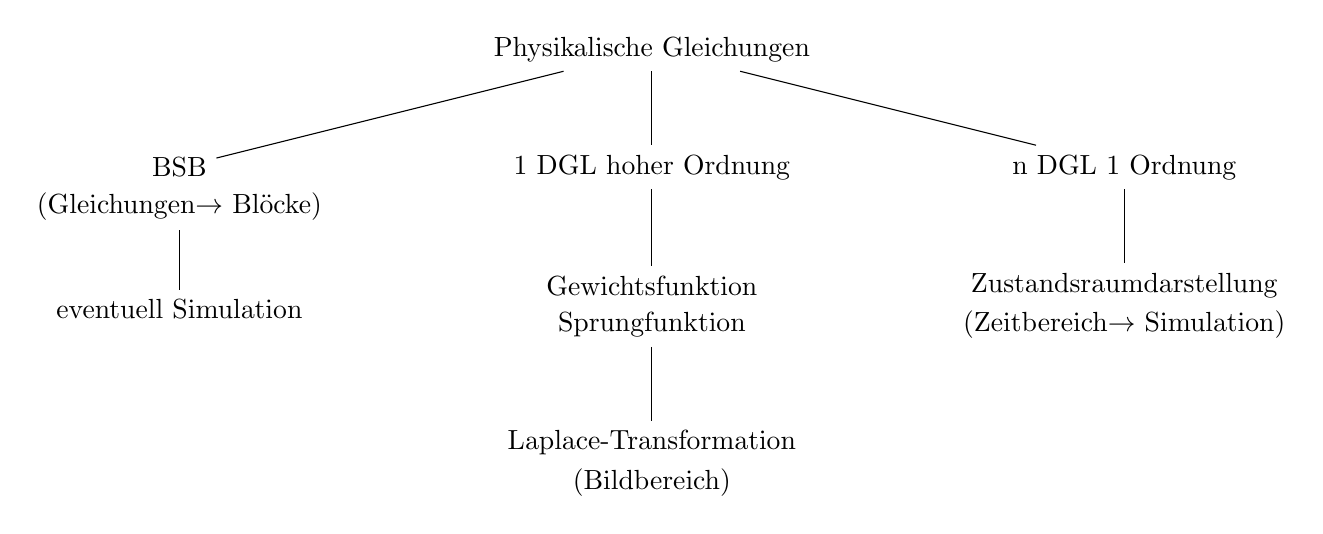
\begin{tikzpicture}
                  \node {Physikalische Gleichungen}
                    child[sibling distance=6cm] {node {BSB}
                     child[level distance=0.5cm]{node {(Gleichungen$\rightarrow$ Blöcke)}edge from parent[draw=none]
                      child[level distance=1.3cm]{node {eventuell Simulation}}
                     }
                  }       
                    child[sibling distance=6cm] {node {1 DGL hoher Ordnung}
                      child {node {Gewichtsfunktion}
                        child[level distance=0.5cm]{node {Sprungfunktion}edge from parent[draw=none]
                         child[level distance=1.5cm]{node{Laplace-Transformation}
                           child[level distance=0.5cm]{node {(Bildbereich)}edge from parent[draw=none]}
}
}
}
}
                    child[sibling distance=6cm] {node {n DGL 1 Ordnung}
                      child {node {Zustandsraumdarstellung}
                         child[level distance=0.5cm]{node {(Zeitbereich$\rightarrow$ Simulation)}edge from parent[draw=none]
                        }
}
                          };
                \end{tikzpicture}
\end{figure}

\subsubsection{Numerische Simulation}

\textbf{gegeben:}
\begin{align*}
  \vec{\dot{x}}(t)=\vec{f}(\vec{x}(t),\vec{u}(t))(*)\\
  \text{Anfangswert } \vec{x}(0)=\vec{x_0}\\
\end{align*}
\textbf{gesucht:} numerische Näherung ${\tilde{x}}$ für die Lösung der DGL auf einem Zeitintervall $[0,t_{max}]$\\
\textbf{Idee: } Approximation von $\vec{\dot{x}}(t)$ durch den Differenzenquotienten:
\begin{equation*}
  \vec{\dot{x}}\approx \frac{\vec{x}(t+h)-\vec{x}(t)}{h} \text{ mit Zeitschritt }h
\end{equation*}
\textbf{Einsetzen in $(*):$ }
\begin{align*}
  \begin{array}{lll}
   \frac{\vec{x}(t+h)-\vec{x}(t)}{h} &\approx& \vec{f}(\vec{x}(t),\vec{u}(t)) \\
   \Rightarrow \vec{x}(t)+h \cdot \vec{f}(\vec{x}(t),\vec{u}(t)) &\approx&x(t+h)
   \end{array}
\end{align*}
mit festen Zeitschritten $t_i=i\cdot h$
\begin{equation*}
  \underbrace{\vec{\tilde{x}}(t_{i+1})}_{\text{neuer Zustand}}=\underbrace{\vec{\tilde{x}}(t_i)}_{\text{alter Zustand}}+h \cdot \vec{f}(\vec{x}(t_i),\vec{u}(t_i))
\end{equation*}
Diese Gleichung lässt sich mithilfe des \emph{Euler-Verfahrens} lösen.

\subsubsection{Lineare Systeme}

\textbf{Fortsetzung Bsp 2.2:}\\
Sortieren der Zustände und der Eingänge:
\begin{align*}
  \begin{array}{lllllllllllll}
    \dot{h_1}(t)&=&-&\frac{C}{A}h_1(t)&+&\frac{C}{A}h_2(t)&&&+&\frac{1}{A}q_1(t)\\
    \dot{h_2}(t)&=&&\frac{C}{A}h_1(t)&-&\frac{2C}{A}h_2(t)&+&\frac{C}{A}h_3(t)\\
    \dot{h_3}(t)&=&&&&\frac{C}{A}h_2(t)&-&\frac{2C}{A}h_3(t)&&&+&\frac{1}{A}q_2(t)
  \end{array}
\end{align*}
Die obige Gleichung lässt sich auch in Vektoren und Matrizen ausdrücken:
\begin{align*}\underbrace{
  \begin{pmatrix}
    \dot{h_1}\\
    \dot{h_2}\\
    \dot{h_3}
  \end{pmatrix}}_{\vec{\dot{x}}(t)}
=
\underbrace{
\begin{pmatrix}
  -\frac{C}{A}&+\frac{C}{A}&0\\
  \frac{C}{A}&-\frac{2C}{A}&\frac{C}{A}\\
  0&\frac{C}{A}&-\frac{2C}{A}
\end{pmatrix}}_{\text{Systemmatrix }\mathbf{A}}
\cdot
\underbrace{
\begin{pmatrix}
h_1(t)\\
h_2(t)\\
h_3(t)  
\end{pmatrix}}_{\parbox{1cm}{\scriptsize Zustands\-vektor~$\vec{x}(t)$}}
+
\underbrace{
\begin{pmatrix}
\frac{1}{A}&0\\
0&0\\
0&\frac{1}{A}  
\end{pmatrix}}_{\parbox{1cm}{\scriptsize Eingangs\-matrix~$\mathbf{B}$}}
\cdot
\underbrace{
  \begin{pmatrix}
    q_1(t)\\
    q_2(t)\\
~
  \end{pmatrix}}_{\parbox{1cm}{\scriptsize Eingangsvektor~$\vec{u}$}}
\end{align*}
Diese Gleichung gilt nur bei linearen Systemen und ist außerdem eine beliebte \textbf{Klausuraufgabe!} Allgemein gilt:
\begin{align*}
  \begin{array}{lllllll}
    \vec{x}(t)&=&\mathbf{A}\cdot\vec{x}(t)&+&\mathbf{B}\cdot\vec{u}(t)&\text{Zustandsdifferentialgleichung}\\
    y(t)&=&\mathbf{C}\cdot \vec{x}(t)&+&\mathbf{B}\cdot\vec{u}(t)&\text{Ausgangsgleichung}
  \end{array}
\end{align*}

\end{document}


 %ENDE DES ZU ERZEUGENDEN DOKUMENTES! AB HIER WIRD BEI DER DOKUMENTERSTELLUNG ALLES IGNORIERT!!

%*******************************************************************
%Es Folgen Copy and Paste Vorlagen für wichtige Anwendungen des	Alltages, wie verschiedene Tabellen etc.
%*******************************************************************
%Einfache Tabelle, die möglichst genau an der eingefügten Stelle im Text auftaucht

\begin{table}[h!]%
\begin{tabular}[h!]{|l||l|l|}stems heißt \emph{Sprungantwort} und wird beschrieben durch
\begin{equation*}
  h(t):=y(t)
\end{equation*}
Mit dem Flächenintegral $y(t)=\int\limits_0^t{g(\tau)\cdot u(t-\tau)d\tau}$ vereinfacht sich das zu
\begin{align*}
  \begin{array}{lll}
    h(t)&=&\int\limits_0^t{g(\tau)\cdot \underbrace{\sigma (t-\tau)}_{=1}d\tau}\\
    h(t)&=&\int\limits_0^t{g(\tau)d\tau}  
  \end{array}
\end{align*}
Die Sprungantwort, genau wie die Gewichtsfunktion, characterisiert das dynamische System vollständig!
\item[Impulsantwort: ] Die Impulsfunktion $\delta (t)$ ist die formale Ableitung des Einheitssprungs.
  \begin{equation*}
    \delta (t)=\frac{d}{dt}\sigma (t) \Leftrightarrow \int\limits_0^t{\delta(\tau)d\tau =\sigma(t)}
  \end{equation*}
Für die Impulsantwort gilt damit:
\begin{equation*}
  \int\limits_0^t{g(\tau)\cdot u(t-\tau)d\tau} =\int\limits_0^t{g(\tau)\cdot \delta(t-\tau)d\tau }=g(t)
\end{equation*}
$\Rightarrow$ Die Gewichtsfunktion $g(t)$ kann auch als Impulsantwort interpretiert werden.

\end{description}

\subsection{Darstellung im Zustandsraum}

\begin{bsp}[System aus 3 verbundenen Wassertanks]
\end{bsp}
\begin{figure}[H]
  \centering
  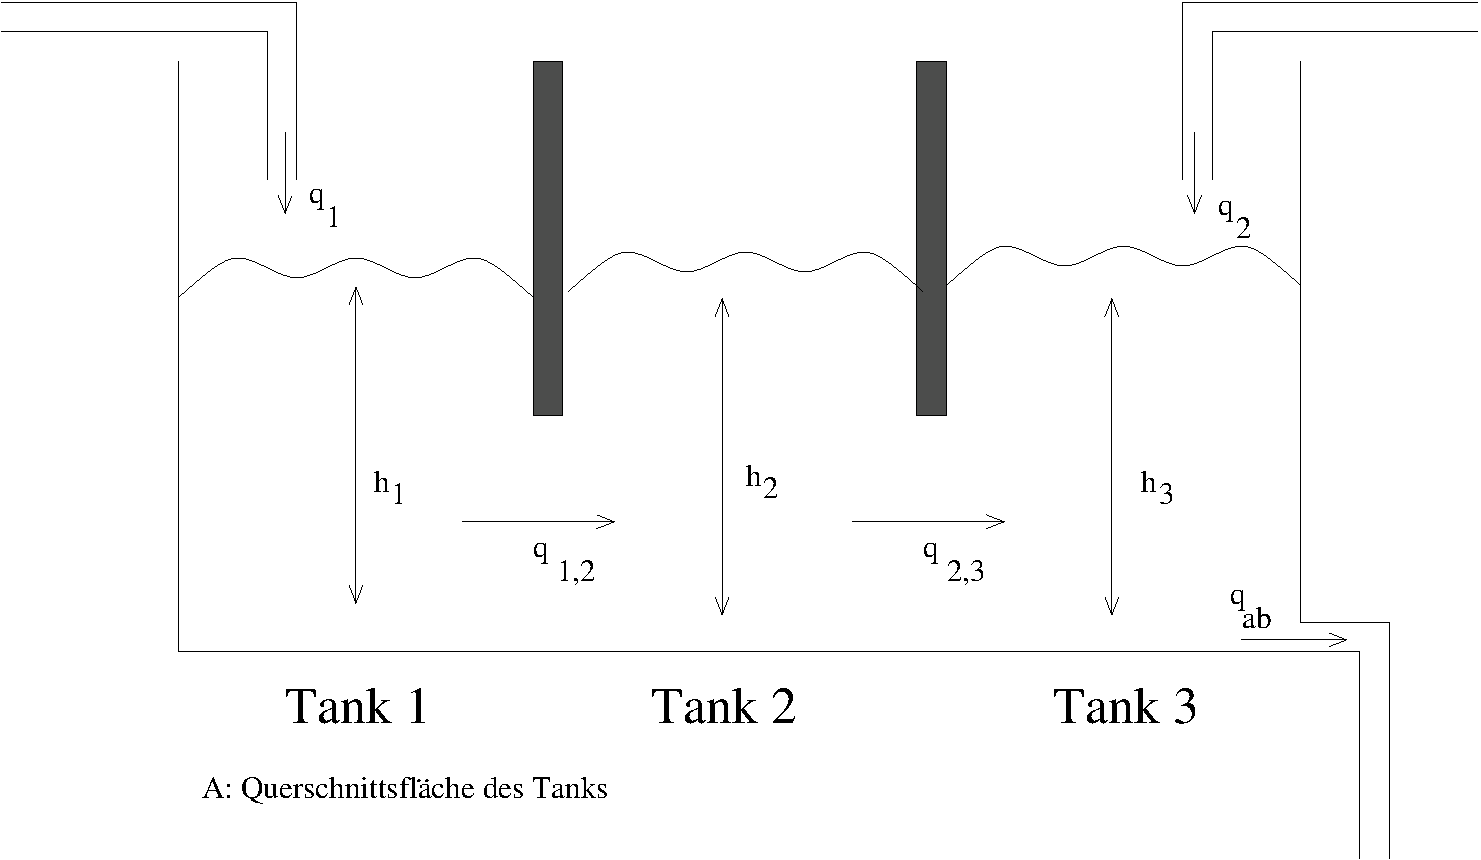
\includegraphics[width=.9\linewidth]{sysregel_bsp_2,2}
\end{figure}
Volumenbilanz:
\begin{align*}
  \begin{array}{llll}
    \text{Tank 1:}&\dot{h_1}&=&\frac{1}{A}(q_1-q_{1,2})\\
    \text{Tank 2:}&\dot{h_2}&=&\frac{1}{A}(q_{1,2}-q_{2,3})\\
    \text{Tank 3:}&\dot{h_3}&=&\frac{1}{A}(q_{2}+q_{2,3}-q_{ab})
  \end{array}
\end{align*}
\begin{description}
\item[Annahme:]Der Ausgleichsfluss zwischen den Tanks ist proportional zur Füllstandsdifferenz: \begin{center}  $q_{1,2}=c\cdot (h_1-h_2);q_{2,3}=c\cdot (h_2-h_3);q_{ab}=ch_3$ \end{center}
\end{description}
\begin{align*}
  \begin{array}{llll}
    \text{damit:}&\dot{h_1}&=&\frac{1}{A}(q_1-ch_1+ch_3)\\
                 &\dot{h_2}&=&\frac{1}{A}(ch_1-2ch_2+ch_3)\\
                 &\dot{h_3}&=&\frac{1}{A}(q_2+ch_2-2ch_3)
  \end{array}
\end{align*}
Kennt man $h_1,h_2,h_3$, so ist der Zustand des Systems zum Zeitpunkt t vollständig bestimmt. $\Rightarrow h_1,h_2,h_3$ sind die Zustandsgrößen des Systems.\\
\textbf{Geometrische Deutung:} $h_1,h_2,h_3$ spannen einen dreidimensionalen Vektorraum auf, den sogenannten \emph{Zustandsraum}.\\
\begin{figure}[H]
  \begin{minipage}{0.5\linewidth}
    \begin{figure}[H]
      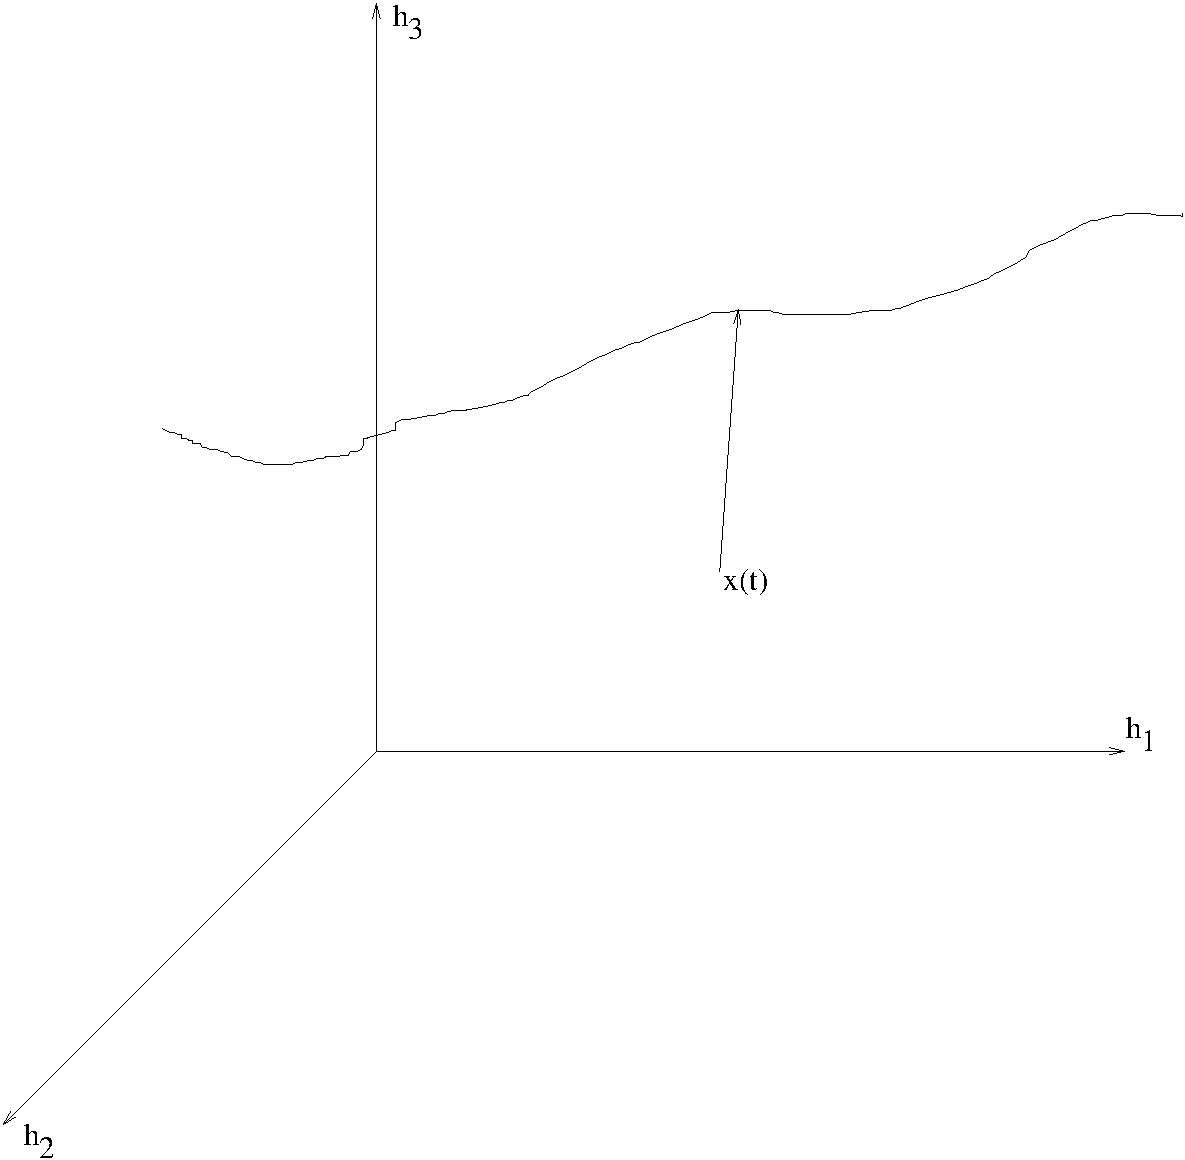
\includegraphics[width=0.9\linewidth]{sysregel_zustandsraum}
    \end{figure}
  \end{minipage}
  \begin{minipage}{0.5\linewidth}
    \[\vec{x}(t): \text{Zustandsvektor}\\\]
    \[\vec{x}(t)=  \begin{pmatrix}
            h_1(t) \\
            h_2(t) \\
            h_3(t) \end{pmatrix} \] 
  \end{minipage}
\end{figure}
Das System wird durch $q_1(t)$ und $q_2(t)$ angeregt, diese sind die \emph{Eingangsgrößen}. Aus ihnen lässt sich der sogenannte \emph{Eingangsvektor} bestimmen:
\begin{equation*}
  \vec{u}(t)=\begin{pmatrix}
                            q_1(t)\\
                            q_2(t)
             \end{pmatrix}
\end{equation*}

\subsubsection*{Verallgemeinerung}

Das Systrem lässt sich durch $n$ Zustände beschreiben:
\[
\vec{x}=
\begin{pmatrix}
x_1\\
x_2\\
\vdots\\
x_n
\end{pmatrix}
\]
Das Systrem besitzt $m$ Eingänge:
\[
\vec{u}=
\begin{pmatrix}
u_1\\
u_2\\
\vdots\\
u_m
\end{pmatrix}
\]
Dieses System lässt sich durch $n$ DGL 1 Ordnung beschreiben:
\[
\left.
\begin{array}{cc}
x_1=f_1(\vec{x},\vec{u})\\
\vdots\\
x_n=f_n(\vec{x},\vec{u})
\end{array}
\right\}
\begin{array}{ll}
\vec{x}(t)=\vec{f}(\vec{x}(t),\vec{u}(t))\\
\text{Zustandsdifferentialgleichung}
\end{array}
\]
Durch Messung des Systems wird aus dem aktuellen Zustand $\vec{x}(t)$ und dem Eingang $\vec{u}(t)$ der Ausgangsvektor $\vec{y}(t)$ bestimmt. Die daraus resultierende Gleichung
\begin{equation*}
  \vec{y}(t)=g(\vec{x}(t),\vec{u}(t))
\end{equation*}
heißt \emph{Ausgangsgleichung}. $\vec{y}(t)$ ist gegeben durch 
\begin{equation*}
  \vec{y}(t)=
\begin{pmatrix}
y_1\\
\vdots\\
y_p
\end{pmatrix}
\end{equation*}
Da man bei komplexen Systemen mit mehreren Ein- und Ausgängen für jedes Eingang/Ausgangpaar eine eigene Gewichtsfunktion aufstellen müsste, bietet sich bei der Simulation solcher Systeme die Zustandsraumdarstellung an.\\  
Die Beschreibung eines Systems im Zustandsraum oder allgemein durch Gleichungen ist der Darstellung im Blockschaubild äquivalent. Je nach Anwendung wird die optimale Beschreibung gewählt. 
%Mindmap ab hier!
\begin{figure}[H]
\centering
                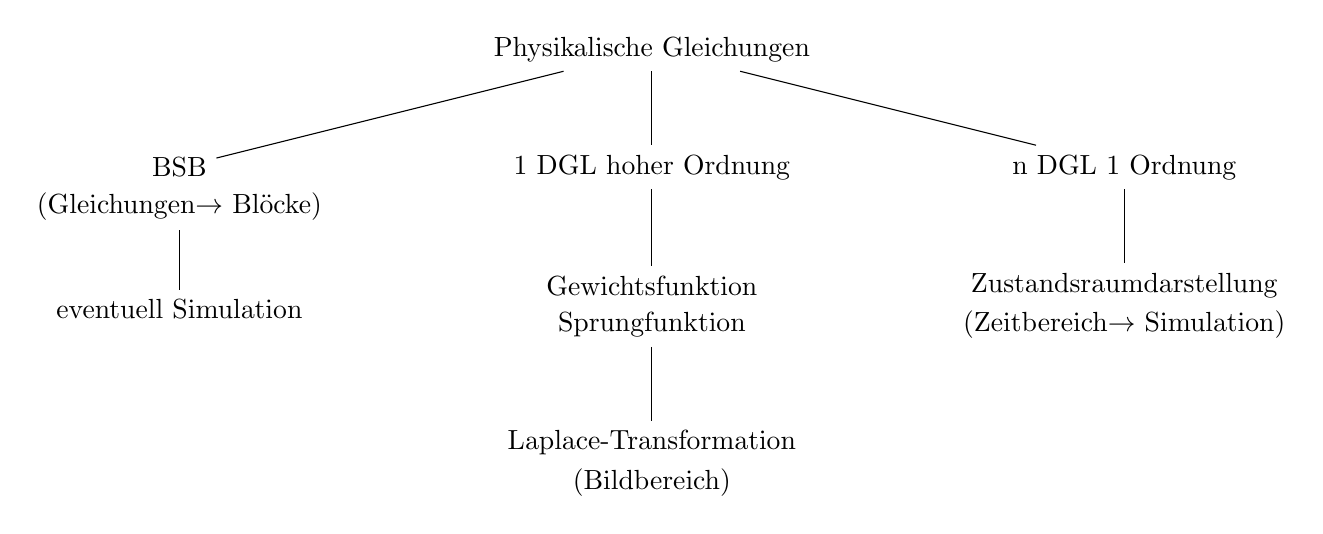
\begin{tikzpicture}
                  \node {Physikalische Gleichungen}
                    child[sibling distance=6cm] {node {BSB}
                     child[level distance=0.5cm]{node {(Gleichungen$\rightarrow$ Blöcke)}edge from parent[draw=none]
                      child[level distance=1.3cm]{node {eventuell Simulation}}
                     }
                  }       
                    child[sibling distance=6cm] {node {1 DGL hoher Ordnung}
                      child {node {Gewichtsfunktion}
                        child[level distance=0.5cm]{node {Sprungfunktion}edge from parent[draw=none]
                         child[level distance=1.5cm]{node{Laplace-Transformation}
                           child[level distance=0.5cm]{node {(Bildbereich)}edge from parent[draw=none]}
}
}
}
}
                    child[sibling distance=6cm] {node {n DGL 1 Ordnung}
                      child {node {Zustandsraumdarstellung}
                         child[level distance=0.5cm]{node {(Zeitbereich$\rightarrow$ Simulation)}edge from parent[draw=none]
                        }
}
                          };
                \end{tikzpicture}
\end{figure}

\subsubsection{Numerische Simulation}

\textbf{gegeben:}
\begin{align*}
  \vec{\dot{x}}(t)=\vec{f}(\vec{x}(t),\vec{u}(t))(*)\\
  \text{Anfangswert } \vec{x}(0)=\vec{x_0}\\
\end{align*}
\textbf{gesucht:} numerische Näherung ${\tilde{x}}$ für die Lösung der DGL auf einem Zeitintervall $[0,t_{max}]$\\
\textbf{Idee: } Approximation von $\vec{\dot{x}}(t)$ durch den Differenzenquotienten:
\begin{equation*}
  \vec{\dot{x}}\approx \frac{\vec{x}(t+h)-\vec{x}(t)}{h} \text{ mit Zeitschritt }h
\end{equation*}
\textbf{Einsetzen in $(*):$ }
\begin{align*}
  \begin{array}{lll}
   \frac{\vec{x}(t+h)-\vec{x}(t)}{h} &\approx& \vec{f}(\vec{x}(t),\vec{u}(t)) \\
   \Rightarrow \vec{x}(t)+h \cdot \vec{f}(\vec{x}(t),\vec{u}(t)) &\approx&x(t+h)
   \end{array}
\end{align*}
mit festen Zeitschritten $t_i=i\cdot h$
\begin{equation*}
  \underbraces{\vec{\tilde{x}}(t_{i+1})}_{\text{neuer Zustand}} =  \underbraces{\vec{\tilde{x}}(t_{i})}_{\text{neuer Zustand}} +h \cdot f(x(t),u(t))
\end{equation*}

\end{document}
\hline 
Funktion & Menge & Gastyp  \\
\hline %Doppelte Linie unter den Überschriften
\hline Ätzgas & 15 sccm & $CF_4$ \\
\hline Passivierungsgas & 35 sccm & $CHF_3$ \\
\hline Physikalische Ätzkomponente & 50 sccm & $Ar$\\
\hline 
\end{tabular}
\caption{Parameter der Ätzung von SiO mit RIE} % Text unter der Tabelle. Nummerierung der Tabelle geschieht automatisch!
\label{tab:RIE-para} % Auf diese Tabelle kann mit "`\ref{tab:RIE-para}"' im Text referenziert werden.
\end{table}

%*******************************************************************
% Zwei zusammenhängende Tabellen nebeneinander, die möglichst an der eingefügten Stelle im Text auftauchen

\begin{table}[h!]
\subfloat[Verwendete Gase\label{tab:DRIE-gas}]{ % Kein "`\caption"' nötig, erstes Argument von Subfloat übernimmt diese Funktion!

\begin{tabular}[b]{|l||l|l|} % [b] = "`Nach Möglichkeit die beiden Tabellenunterschriften auf einer Höhe halten!

\hline Funktion & Menge & Gastyp\\
\hline %Doppelte Linie unter den Übverschriften
\hline Ätzgas & 130 sccm & $SF_6$\\
\hline Zusatz zum Ätzgas & 12 sccm & $O_2$\\
\hline Passivierungsgas & 85 scm & $C_4F_8$ \\
\hline
\end{tabular}
}
\subfloat[Daten der Ätzzyklen\label{tab:DRIE-cycle}]{% Auf diese Tabelle kann mit "`\ref{tab:DRIE-Cycle}"' im Text referenziert werden.
\begin{tabular}[b]{|l|l|}
\hline Anzahl Zyklen & 61 \\
\hline
\hline Dauer Ätzteilzyklus & 13 sec \\
\hline Dauer Passivierungsteilzyklus & 7 sec \\
\hline Dauer Gesamtzyklus & 20 sec \\
\hline
\end{tabular}
}
\caption{Parameter der Ätzung mit DRIE} % Dieser Caption erstreckt sich unter BEIDEN Tabellen und ist eine GESAMTÜBERSCHRIFT der Tabellenkombination! 
\label{tab:DRIE-para}% Auf diese Tabellenkombination kann mit "`\ref{tab:DRIE-para}"' im Text referenziert werden.
\end{table}

%*******************************************************************
%Bild neben einer Tabelle

\begin{figure}[h]
  \begin{minipage}{.45\linewidth} %Anfang Bildbereich, 0,45 % der Seitenbreite
\includegraphics[height=5.5cm]{messpkt} % Hier Bild einfügen
\caption{Position der Messpunkte} %Bildunterschrift
\label{pic:messpkt} %Referenzieren mittels "`\ref{pic:messpkt}"'
 \end{minipage}% Ende des Bildbereiches
 
 \begin{minipage}{.55\linewidth} %Anfang Tabellenbereich, 0,55 % der Seitenbreite
\begin{tabular}[h]{|l|l|l|}
\hline Anzahl Zyklen & 61 \\
\hline
\hline Dauer Ätzteilzyklus & 13 sec \\
\hline Dauer Passivierungsteilzyklus & 7 sec \\
\hline Dauer Gesamtzyklus & 20 sec \\
\hline
\end{tabular}
\captionof{table}{Daten DRIE-Zyklus} % Tabellenunterschrift, mit \captionof{table} einzufügen, da wir uns in der "`figure"' Umgebung befinden!
\label{tab:Cyc} %Referenzieren mit "`\ref{tab:Cyc}"'
\end{minipage}% Ende des Tabellenbereiches
\end{figure}

%*******************************************************************
%Tabelle mit einer Spalte, die mehrere Zeilen umfassen kann.

\begin{table}  
\begin{tabular}[h]{|c|l|l|}
\hline Messpunkt & Strukturbreite & Ätztiefe\\
\hline 
\multirow{2}{*}{1} % Syntax: \multirow{ANZAHL ÜBERSPANNTER REIHEN}{*}{INHALT}
& $100~ \micro m$ & $42,5~ \micro m$  \\  \cline{2-3} 
& $20~ \micro m$  & $31,0~ \micro m$  \\  \hline
\multirow{2}{*}{2} 
& $100~ \micro m$ & $44,0~ \micro m$  \\  \cline{2-3} 
& $20~ \micro m$  & $30,0~ \micro m$  \\  \hline
\multirow{2}{*}{3}  
& $100~ \micro m$ & $36,5~ \micro m$  \\  \cline{2-3} 
& $20~ \micro m$  & $27,0~ \micro m$  \\  \hline
\multirow{2}{*}{Durchschnitt} 
& $100~ \micro m$ & $41,0~ \micro m$  \\  \cline{2-3} 
& $20~ \micro m$  & $29,3~ \micro m$  \\  \hline
\multirow{2}{*}{Standardabweichung} 
& $100~ \micro m$ & $1,5~ \micro m$  \\  \cline{2-3} 
& $20~ \micro m$  & $2,0~ \micro m$  \\  \hline
\end{tabular}
\caption{Gemessene Ätztiefen an 3 Punkten}
\label{tab:struk} %Referenzieren mittels "`\ref{tab:struk}"'
\end{table}

%*******************************************************************
%Literatur- und Quellenverzeichniss

\begin{thebibliography}{sotief} % {sotief} bestimmt die Einrücktiefe der einzelnen Elemente (Breite des in den geschweiften Klammern stehender Text = Einrücktiefe!)

\bibitem{mst}R. Zengerle, Mikrosystemtechnik: Technologien und Prozesse, Skript zur Vorlesung, Kapitel 6 (Ätzen) und Kapitel 7 (OMM) %Auf dieses Werk wird im Text über "`\ref{mst} referenziert

\end{thebibliography}

%*******************************************************************